% Template file for an a0 landscape poster.
% Written by Graeme, 2001-03 based on Norman's original microlensing
% poster.
%
% See discussion and documentation at
% <http://www.astro.gla.ac.uk/users/norman/docs/posters/> 
%
% $Id: poster-template-landscape.tex,v 1.2 2002/12/03 11:25:46 norman Exp $


% Default mode is landscape, which is what we want, however dvips and
% a0poster do not quite do the right thing, so we end up with text in
% landscape style (wide and short) down a portrait page (narrow and
% long). Printing this onto the a0 printer chops the right hand edge.
% However, 'psnup' can save the day, reorienting the text so that the
% poster prints lengthways down an a0 portrait bounding box.
%
% 'psnup -w85cm -h119cm -f poster_from_dvips.ps poster_in_landscape.ps'

\documentclass[a0]{a0poster}
% You might find the 'draft' option to a0 poster useful if you have
% lots of graphics, because they can take some time to process and
% display. (\documentclass[a0,draft]{a0poster})
\input defs
\pagestyle{empty}
\setcounter{secnumdepth}{0}
\renewcommand{\familydefault}{\sfdefault}
\newcommand{\QED}{~~\rule[-1pt]{8pt}{8pt}}\def\qed{\QED}

\renewcommand{\reals}{{\mbox{\bf R}}}

% The textpos package is necessary to position textblocks at arbitary 
% places on the page.
\usepackage[absolute]{textpos}

\usepackage{fleqn,psfrag,wrapfig,tikz}
\usepackage{enumitem}
\usepackage{amsmath}

\usepackage{caption}

%\usepackage{svg}
\usepackage[papersize={38in,28in}]{geometry}

% Graphics to include graphics. Times is nice on posters, but you
% might want to switch it off and go for CMR fonts.
\usepackage{graphics}

% we are running pdflatex, so convert .eps files to .pdf
%\usepackage[pdftex]{graphicx}
%\usepackage{epstopdf}

% These colours are tried and tested for titles and headers. Don't
% over use color!
\usepackage{color}
\definecolor{Red}{rgb}{0.9,0.0,0.1}

\definecolor{bluegray}{rgb}{0.15,0.20,0.40}
\definecolor{bluegraylight}{rgb}{0.35,0.40,0.60}
\definecolor{gray}{rgb}{0.3,0.3,0.3}
\definecolor{lightgray}{rgb}{0.7,0.7,0.7}
\definecolor{darkblue}{rgb}{0.2,0.2,1.0}
\definecolor{darkgreen}{rgb}{0.0,0.5,0.3}

\renewcommand{\labelitemi}{\textcolor{bluegray}\textbullet}
\renewcommand{\labelitemii}{\textcolor{bluegray}{--}}

\setlength{\labelsep}{0.5em}


% see documentation for a0poster class for the size options here
\let\Textsize\normalsize
%\def\Head#1{\noindent\hbox to \hsize{\hfil{\LARGE\color{bluegray} #1}}\bigskip}
\def\Head#1{\noindent{\LARGE\color{bluegray} #1}\bigskip}
\def\LHead#1{\noindent{\LARGE\color{bluegray} #1}\bigskip}
\def\Subhead#1{\noindent{\large\color{bluegray} #1}\bigskip}
\def\Title#1{\noindent{\VeryHuge\color{Red} #1}}


% Set up the grid
%
% Note that [40mm,40mm] is the margin round the edge of the page --
% it is _not_ the grid size. That is always defined as 
% PAGE_WIDTH/HGRID and PAGE_HEIGHT/VGRID. In this case we use
% 23 x 12. This gives us three columns of width 7 boxes, with a gap of
% width 1 in between them. 12 vertical boxes is a good number to work
% with.
%
% Note however that texblocks can be positioned fractionally as well,
% so really any convenient grid size can be used.
%
\TPGrid[40mm,40mm]{23}{12}      % 3 cols of width 7, plus 2 gaps width 1

\parindent=0pt
\parskip=0.2\baselineskip

\begin{document}

% Understanding textblocks is the key to being able to do a poster in
% LaTeX. In
%
%    \begin{textblock}{wid}(x,y)
%    ...
%    \end{textblock}
%
% the first argument gives the block width in units of the grid
% cells specified above in \TPGrid; the second gives the (x,y)
% position on the grid, with the y axis pointing down.

% You will have to do a lot of previewing to get everything in the 
% right place.

% This gives good title positioning for a portrait poster.
% Watch out for hyphenation in titles - LaTeX will do it
% but it looks awful.
\begin{textblock}{23}(0,0)
\Title{Neon: Nuclear Norm to Beat Muon}
\end{textblock}

\begin{textblock}{23}(0,0.6)
{
\LARGE
Alexey Kravatskiy, Ivan Kozyrev, Nikolay Kozlov, Alexander Vinogradov
}

{
\Large
\color{bluegray}
\emph{Optimization Class Project. MIPT}
}
\end{textblock}


% Uni logo in the top right corner. A&A in the bottom left. Gives a
% good visual balance, but you may want to change this depending upon
% the graphics that are in your poster.
%\begin{textblock}{2}(0,10)
%Your logo here
%%\includegraphics{/usr/local/share/images/AandA.epsf}
%\end{textblock}

%\begin{textblock}{2}(21.2,0)
%Another logo here
%%\resizebox{2\TPHorizModule}{!}{\includegraphics{/usr/local/share/images/GUVIu/GUVIu.eps}}
%\end{textblock}


\begin{textblock}{7.0}(0,1.5)

\hrule\medskip
\Head{Introduction}\\
Recent advances in optimization techniques have highlighted the benefits of leveraging the matrix structure of neural network weights during training. Optimizers like Muon (Jordan et al.) and Shampoo (Gupta, Koren and Singer) have shown promise, but at a significantly higher computational cost than traditional methods like Adam. To bridge this gap, we propose Neon, a new optimizer that builds upon the framework of Bernstein and Newhouse. By using alternative norms, such as kernel norm (Kernel-Neon) or custom $F*$ norm ($F*$-Neon), we induce low-rank update matrices that enable more efficient computation. We evaluate the performance of Neon, Muon, and Adam on MLP, CIFAR10, and NanoGPT, and demonstrate [resting results here].

\medskip
\hrule\medskip
\Head{Neon's update rule}\\
Bernstein and Newhouse suggest obtaining the update step for a weight matrix $W$ as a solution to the optimization problem:
\begin{equation}
    \langle G, \delta W \rangle + \frac{\lambda}{2} \norm{\delta W}^2 \to \min_{\delta W}\,,
\end{equation}
where $G$ is a gradient-like matrix obtained via backpropagation. Setting norm to RMS-to-RMS norm (scaled version of Spectral norm) produces Muon. We consider two different choices instead:
\begin{enumerate}
    \item Choosing kernel norm, $\norm{\cdot}_*$, produces rank-1 update, defined by 
    \begin{equation}\label{eqn:update_star}
        \delta W = -\frac{1}{\lambda} u_1 \sigma_1 v_1^T\,,
    \end{equation}
    where $\sigma_1$ is largest singular value of $G$, and $u_1$, $v_1$ are corresponding singular values.

    \item Choosing $F*$ norm, defined by $\norm{\cdot}_{F*} = (\norm{\cdot}_{*} + \norm{\cdot}_{F})/2$, produces a relatively small-rank update, defined by
    \begin{equation}\label{eqn:update_F_star}
    \delta W = -\frac{1}{\lambda}UDV^T
    \end{equation} 
    with $D = \diag(d_i)$, where $d_i = [\sigma_i - \tau]_+$ and $\tau$ is given by
    \begin{equation*}
        \sum_{i=1}^n [\sigma_i - \tau]_+ = \tau\,.
    \end{equation*}
\end{enumerate}

\medskip
\hrule\medskip
\Head{Efficient update computation}\\
% A couple of sentences about Lanczos algorithm and reference computation times and required number of iterations for tipical value of $\tau$.
We use cupy's svds routine to obtain gradients' matrices' SVD approximation formed by largest singular values and corresponding vectors.
By applying the Lanczos process to either $A^TA$ or $AA^T$, it generates a sequence of orthogonal vectors (Lanczos vectors) that capture 
the dominant spectral properties of the original matrix. The singular values and vectors are then extracted from the tridiagonal matrix using 
standard eigenvalue techniques like QR iteration.
\end{textblock}

\begin{textblock}{7.0}(8,1.5)
\hrule\medskip
\Head{Algorithms}\\
Now we can write down pseudocode for both versions of Neon.

\noindent\rule[-5pt]{.8\textwidth}{0.4pt}\\
{\bf Algorithm 1} Kernel-Neon update step for linear layer\\
\noindent\rule[10pt]{.8\textwidth}{0.4pt}
\vspace{-10pt}
\noindent\begin{tabbing}
    {\bf Input:} $\lambda$, gradient-like matrix $G$. \\
    {\bf Output:} Weight matrix update $\delta W$.\\*[\smallskipamount]
    \qquad \= 1.\ $U, \Sigma, V := \textrm{Lanczos}(G, 1)$. \\
    {\bf Return} $-\frac{1}{\lambda}U \Sigma V^T$.
\end{tabbing}
\vspace{-8pt}
\noindent\rule[10pt]{.8\textwidth}{0.4pt}

For $F*$-Neon it is a bit trickier~\eqref{eqn:update_F_star}, we need to compute $\tau$ and know number of singular values larger then $\tau$, which we denote by $r$. Assuming that singular values spectrum of $G$ changes little between iterations (which was true in our experiments) we propose the following algorithm.

\noindent\rule[-5pt]{.8\textwidth}{0.4pt}\\
{\bf Algorithm 2} $F*$-Neon update step for linear layer\\
\noindent\rule[10pt]{.8\textwidth}{0.4pt}
\vspace{-10pt}
\noindent\begin{tabbing}
    \qquad\=\qquad\=\qquad\=\kill % Set three tab stops (4em total)
    {\bf Input:} $\lambda$, $r$, gradient-like matrix $G$. \\
    {\bf Output:} Weight matrix update $\delta W$.\\*[\smallskipamount]
    \> 1. $U, \Sigma, V := \textrm{Lanczos}(G, r + 1)$. \\
    \> 2. $s := \sum_{i=1}^{r}\sigma_r$. \\
    \> 3.\ {\bf If} $(r + 1)\sigma_{r + 1} > s${\bf:}\\
    \>\> 4. $r := r + 1$. 5. $\tau := \frac{s + \sigma_{r}}{r + 1}$.\\
    \> 6.\ {\bf Else if} $(r + 1)\sigma_{r - 1} < s${\bf:}\\
    \>\> 7. $r := r - 1$. 8. $\tau := \frac{s - \sigma_{r}}{r + 1}$.\\
    \> 9.\ {\bf Else:}\\
    \>\> 10. $\tau := \frac{s}{r + 1}$\\
    \> 11. $D = [\Sigma - \tau I]_+$. \\*[\smallskipamount]
    {\bf Save} $r$ for the next iteration.\\
    {\bf Return} $-\frac{1}{\lambda}U D V^T$.
\end{tabbing}
\vspace{10pt}
%\noindent\rule[10pt]{.8\textwidth}{0.4pt}

\hrule\medskip
\Head{MLP tests}\\
We test Muon, SGD, and Neon on a simple MLP (2 linear layers) that solves CIFAR-10 classification problem. Muon converges faster than Neon and reaches higher accuracy.
\begin{figure}[h]
    \center{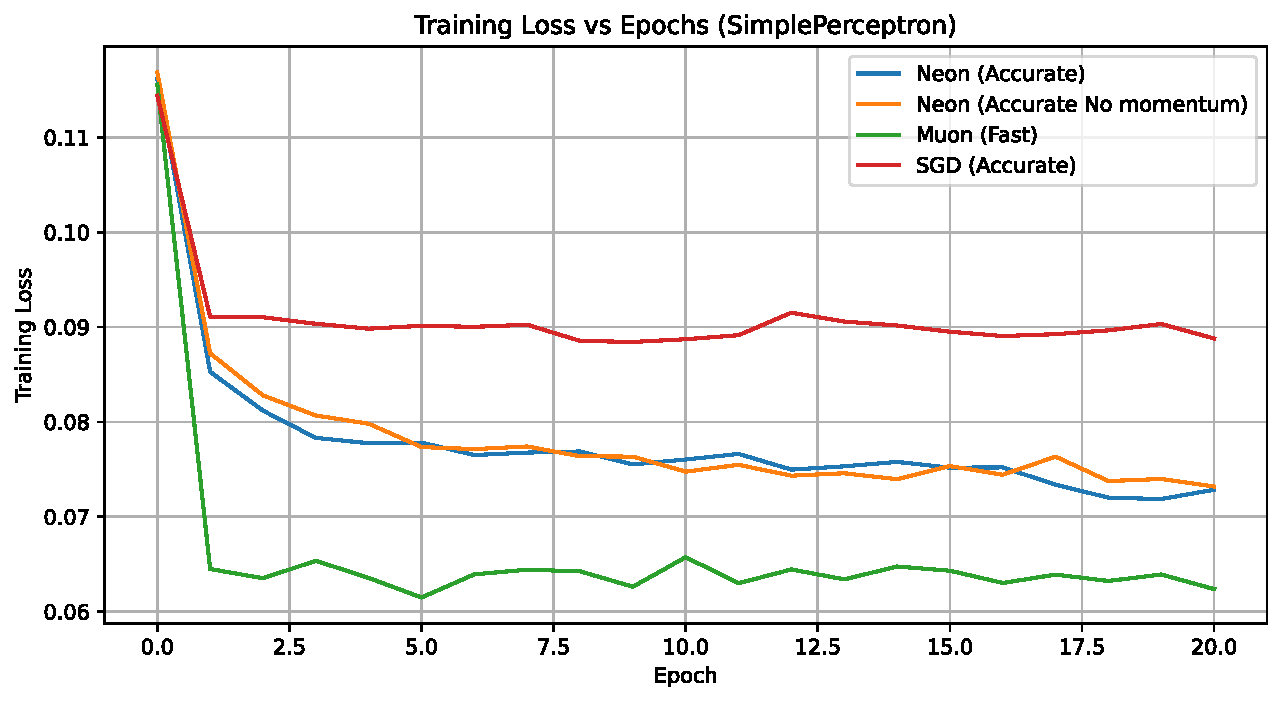
\includegraphics[width=0.8\linewidth]{../figs/mlp0605/loss_vs_epochs_mlp.pdf}}
    \caption{MLP validation loss}
    \label{fig:mlp_loss}
\end{figure} 


\end{textblock}

\begin{textblock}{7.0}(16,1.5)
    \begin{figure}[h]
        \center{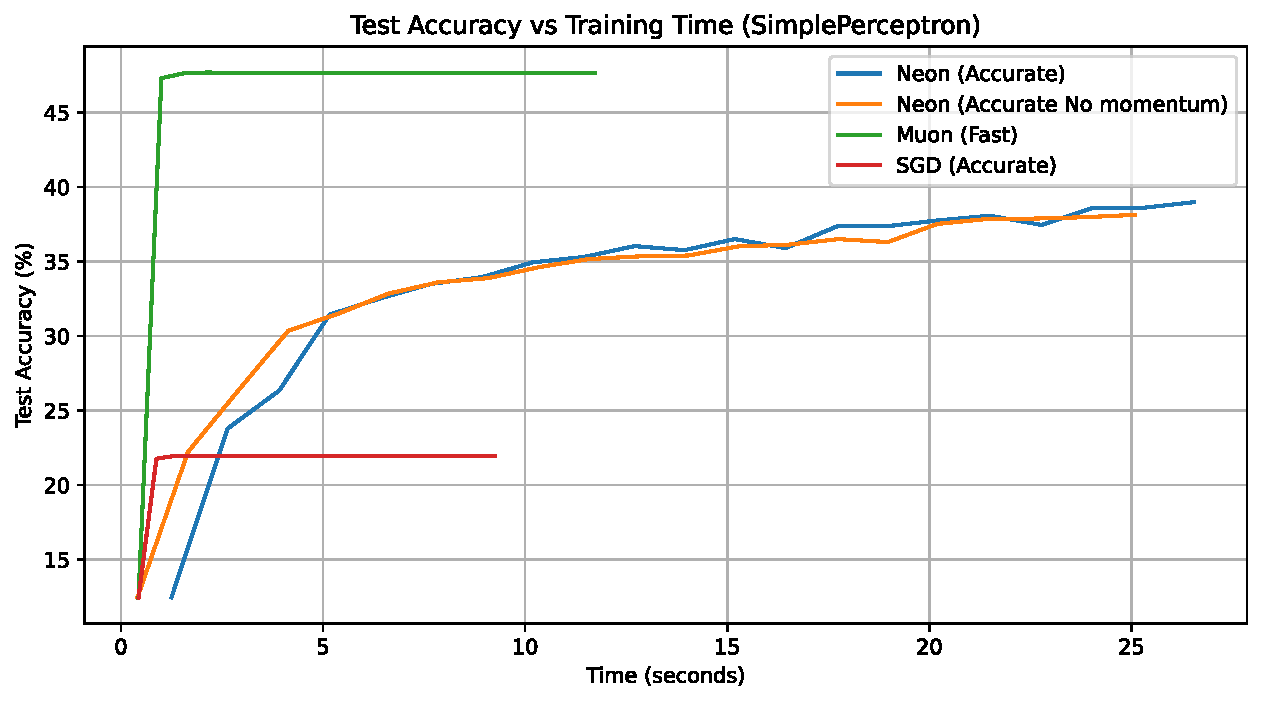
\includegraphics[width=0.8\linewidth]{../figs/mlp0605/accuracy_vs_time_mlp.pdf}}
        \caption{MLP Accuracy vs wallclock time}
        \label{fig:mlp_loss}
    \end{figure} 

\hrule\medskip
\Head{CIFAR-10 tests}\\
Now we compare Muon and Neon on ResNet from Keller's cifar10-aribench at GitHub. On RTX-4050, Muon is approximately twice as fast as Neon. Moreover, Neon has a strange dependency on batch size that has not been observed for Muon: smaller batch size 500 leads to accuracy 84\% in eight epochs, while batch size 2000 results in only 51\%.

TO-DO: we conduct experiments like those with MLP, and add plots here.


\medskip
\hrule\medskip
\Head{NanoGPT tests}\\
Couple of sentences and a vector(!) picture (reference picture for now).
% \begin{figure}[h]
%     \center{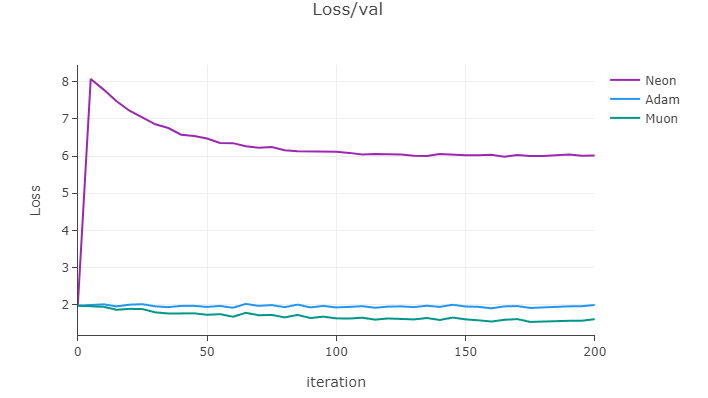
\includegraphics[width=0.8\linewidth]{../figs/mlp24/loss_val.png}}
%     \caption{NanoGPT validation loss}
%     \label{fig:nanogpt_loss}
% \end{figure} 
% \begin{figure}[h]
%     \center{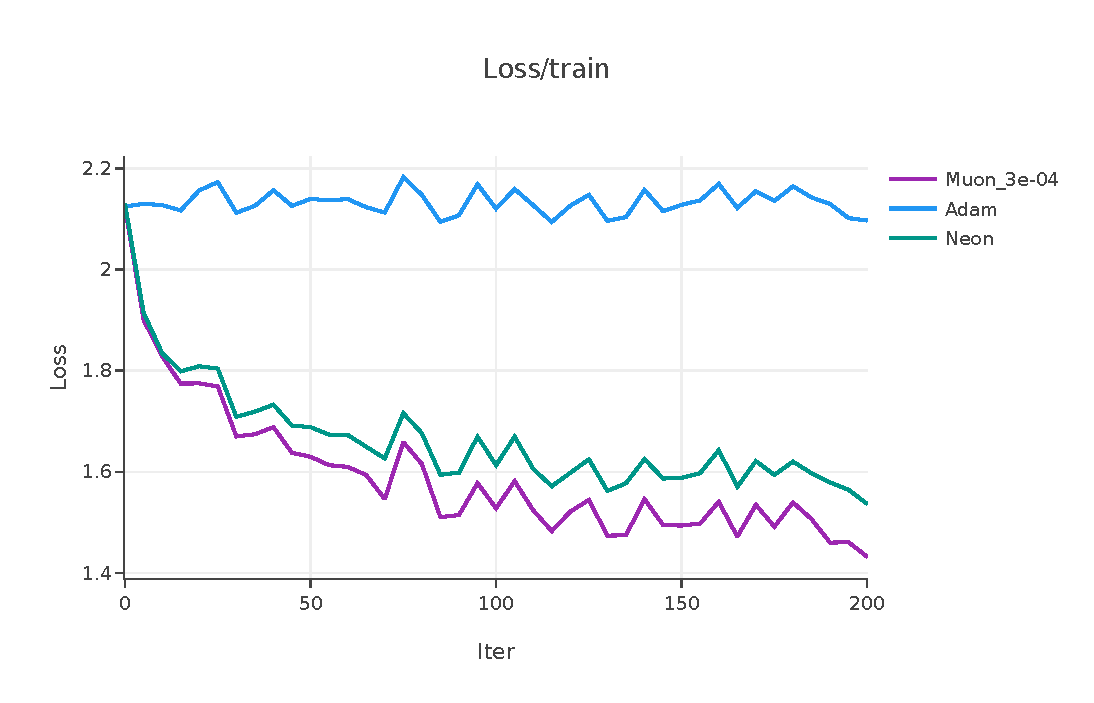
\includegraphics[width=0.8\linewidth]{../figs/nanogpt/train_loss.pdf}}
%     \caption{NanoGPT train loss}
%     \label{fig:nanogpt_train_loss}
% \end{figure}
\begin{figure}[h]
    \center{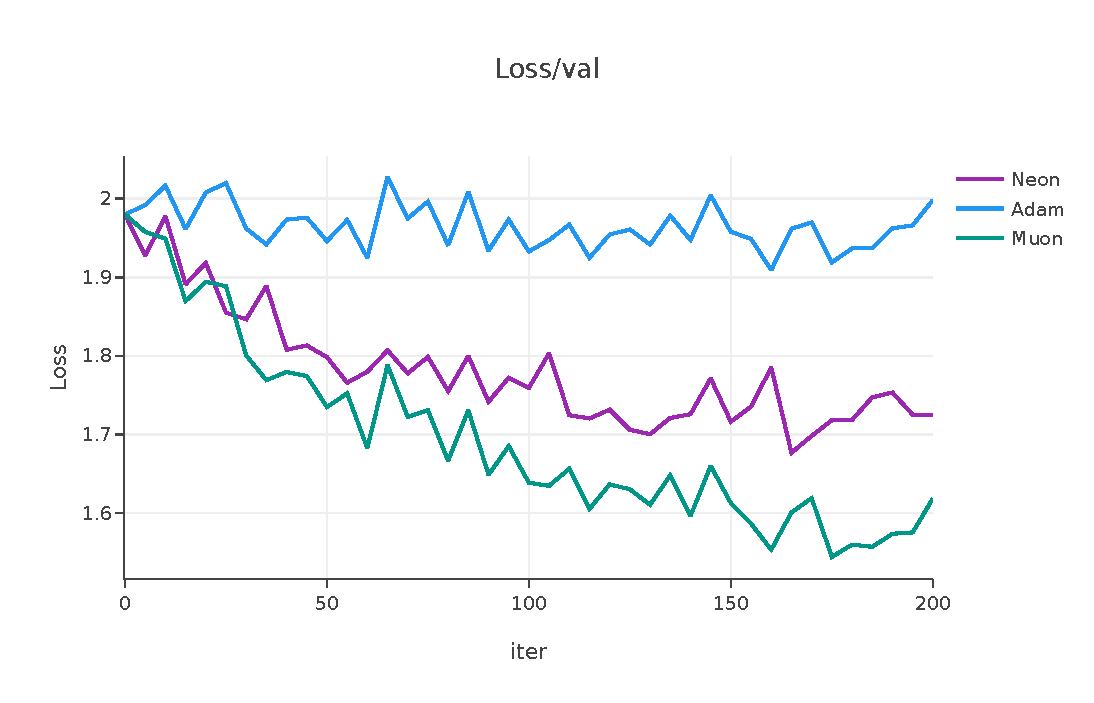
\includegraphics[width=0.8\linewidth]{../figs/nanogpt/val_loss.pdf}}
    \caption{NanoGPT validation loss}
    \label{fig:nanogpt_val_loss}
\end{figure}
\medskip
\hrule\medskip
\Head{Conclusion}\\
Lorem ipsum dolor sit amet, consectetur adipisicing elit, sed do eiusmod tempor incididunt ut labore et dolore magna aliqua. Ut enim ad minim veniam, quis nostrud exercitation ullamco laboris nisi ut aliquip ex ea commodo consequat. Duis aute irure dolor in reprehenderit in voluptate velit esse cillum dolore eu fugiat nulla pariatur. Excepteur sint occaecat cupidatat non proident, sunt in culpa qui officia deserunt mollit anim id est laborum.

\medskip
\hrule\medskip
\Head{Acknowledgements}\\
This material is based upon work supported by the
X Fellowship and my mom.

\end{textblock}

\end{document}